\section{一维运动的一般性质}\label{sec:06.05}

现在我们讨论一维运动。例如沿着直线的运动,并假定力是
保守的用$ x $表示位置坐标。

由一维情况功与力的关系式\ref{eqn:06.02.06}
\begin{equation*}
  A _ { 1 \to 2 } = \int _ { x _ { 1 }} ^ { x _ { 2 } } F  \dif x
\end{equation*}\label{err:06.05.01}
以及力是保守的,即
\begin{align*}
  &A _ { 1 \to 2 } = V \left( x _ { 1 } \right) - V \left( x _ { 2 } \right) \\
  \beforetext{有} &V \left( x _ { 1 } \right) - V \left( x _ { 2 } \right) = \int _ { x _ { 1 }} ^ { x _ { 2 } } F \dif x
\end{align*}\label{err:06.05.02}
由此可知,一维情况下的保守力$ F $可表示为
\begin{equation}\label{eqn:06.05.01}
  F = - \frac { \dif V } { \dif x }
\end{equation}
或者,凡是能表示成式\eqref{eqn:06.05.01}形式的力一定是保守力。例如,对于%
% 183.jpg
\clearpage\noindent%
自由落体运动,如果取坐标$ x $为从地面算起的高度,则
其势能函数分别为
\begin{equation*}
  F = - m g  \qquad V = m g x + V _ 0
\end{equation*}
其中$ V _ 0  $为任意常数。由选择势能的零点所确定。若选择地面(即
$ x = 0 $)处的势能为零,则$  V _ { 0 } = 0  $ 。

一维情况的质点的机械能守恒,有下列的形式:
\begin{equation}\label{eqn:06.05.02}
  \frac { 1 } { 2 } m \left( \frac { \dif x } { \dif t } \right) ^ { 2 } + V \left( x \right) = E
\end{equation}
由于质点的动能
$ \dfrac { 1 } { 2 } m \left( \dfrac { \dif x } { \dif t } \right) ^ { 2 }  $
不能为负值,所以上式给我们一个不等式
\begin{equation}\label{eqn:06.05.03}
  E \geqslant V \left( x \right)
\end{equation}
这个不等式的物理意义是很显然的,它表示质点的总能量总是大
于或等于势能。根据这个论断,只要知道了势能函数$ V\left(x\right) $以及质
点的能量,不必详细求解运动方程,质点的运动范围就完全确定
了。下面举例说明。

设质点的势能函数$  V \left( x \right)   $如图\ref{fig:06.12}所示,这种曲线常称为势能
\begin{figure}[h]
    \centering
    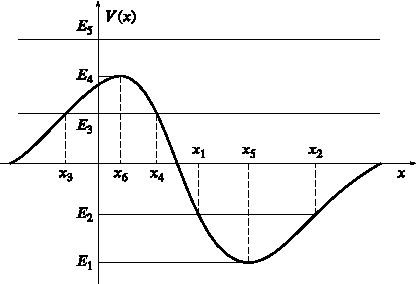
\includegraphics{figure/fig06.12}
    \caption{势能函数及运动性质}
    \label{fig:06.12}
    \vspace{-0.8em}
\end{figure}
% 184.jpg
\clearpage\noindent
曲线,图\ref{fig:06.02}中的$ mgz $线就是重力势能曲线。


由图\ref{fig:06.12},如果质点的能量$ E=E_2 $,则不等式\eqref{eqn:06.05.03}要求$x _ 1
    < x < x _ 2$,这表示具有能量$ E_2 $的质点只能在$ x_1 $与$ x_2 $之间运动,$ x_1 $与
$ x_2 $是方程$ V \left(x\right) = E_2 $的两个根。这种在有限范围中的运动称为束
缚运动。对于图\ref{fig:06.12}所表示的势能函数,当质点能量在$ E_1 \leqslant E \leqslant 0 $时,都是作束缚运动。

当质点能量$  E > 0  $时,运动范围可以延伸到无限远。例如,当
$ E = E _ 3 $时,质点可以在$ -\infty < x \leqslant x_3 $,或者$ x_4 \leqslant x < \infty $两个无限的
范围中运动,其中$ x_3 $,$ x_4 $是方程$  V \left( x \right) = E _ { 3 }   $的两个根。当$  E = E _ 5  $,
时,质点可以在整个$ x $的范围,即$  - \infty < x < \infty   $中运动。这种具有
无限范围的运动,称为非束缚的,或自由运动。

对于$  E = E _ 3  $情况,如果开始时质点在$  x > x _ { 4 }   $的范围中运动,
则它永远不会跑到$ x < x_3 $的范围中去。因为从$  x > x _ { 4 }   $到$  x < x _ 3 $,必
须经过$ x_3 < x < x_4 $,而这一范围质点是不可能进入的。所以,对于
能量为$ E_3 $的质点来说,势能函数的作用相当于在$  x _ { 3 } < x < x _ { 4 } $范围
中造成一个不可逾越的壁垒,常称为势垒。

当$  E = E _ 1 $时,质点只能处于$ x = x_5 $点,它的动能为零,速度为
零,所以,这是静止的质点。从受力的角度来分析,由于$ x = x_5 $
是$ V\left(x\right) $的极小点,故有
\begin{equation*}
  F \left( x _ { 5 } \right) = - \left( \frac { \dif v } { \dif x } \right) _ { x _ 5 } = 0
\end{equation*}
即处在$ x = x_5 $的质点并不受力。所以,它能保持速度为零的状态,
即静止的状态。

当质点处于$ x = x_6 $时,同样有
\begin{equation*}
  F \left( x _ { 6 } \right) = - \left( \frac { \dif v } { \dif x } \right) _ { x _ 6 } = 0
\end{equation*}
也是不受力的。因此,对于能量为$  E _ { 4 } = V \left( x _ { 6 } \right)   $的质点,在$  x = x _ { 6 }  $
处的动能为零,速度为零,并也能保持速度为零的状态不变,处
% 185.jpg
于静止。

但是,$  E = E _ { 1 }   $,及$  E = E _ 4 $两种静止状态是十分不同的。在前
一情况,不等式\eqref{eqn:06.05.03}要求质点只能处于$  x = x _ { 5 } $;而在后一情况,
质点可以处于$ - \infty < x < \infty   $整个范围。所以,前一种静止状态是
稳定的,它不可能离开静止状态;后一种静止是不稳定的,它可
以偏离静止变成运动状态。

讨论了运动范围之后,我们来讨论运动解。

由式\eqref{eqn:06.05.02},可以得到
\begin{equation*}
  \frac { \dif x } { \dif t } = \pm \sqrt { \frac { 2 } { m } \left( E - V \left( x \right) \right) }
\end{equation*}
正号和负号分别表示沿正$ x $及负$ x $方向的运动。积分上式,就得到
\begin{equation}\label{eqn:06.05.04}
  t = \pm \sqrt { \frac { m } { 2 } } \int _ { x _ { 0 } } ^ { x } \frac { \dif x } { \sqrt { E - V \left( x \right) } }
\end{equation}
利用上式可以求出作束缚运动的质点从$ x_1 $到$ x_2 $(图6.12)所用的
时间,即
\begin{equation}\label{eqn:06.05.05}
  \sqrt { \frac { m } { 2 } } \int _ { x _ { 1 } } ^ { x _ { 2 } } \frac { \dif x } { \sqrt { E _ { 2 } - V \left( x \right) } }
\end{equation}
当质点到了$ x_2 $,它的速度变为零,因为$  E _ { 2 } = V \left( x _ { 2 } \right)   $。但在$ x_2 $点,
$ \dfrac { \dif V } { \dif x } > 0   $
,所以,$  F < 0  $,即力是指向负$ x $方向的,这个力使质点
发生沿着负$ x $方向运动,也就是说,力使质点在$ x_2 $处改变运动
方向,质点从$ x_2 $回到$ x_1 $所用的时间为
\begin{equation}\label{eqn:06.05.06}
  - \sqrt { \frac { m } { 2 } } \int _ { x _ { 2 } } ^ { x _ { 1 } }  \frac { \dif x } { \sqrt { E _ { 2 } - V \left( x \right) } }
\end{equation}
根据上述类似的讨论可知,质点到达$ x_1 $后,运动方向也发生变
化,从负$ x $方向变为正$ x $方向。总之,束缚运动是质点在$ x_1 $与$ x_2 $
之间来回振荡的运动。质点完成一个运动循环(从$ x_1 $到$ x_2 $再回到$
  x _ { 1 } $)的时间,称为周期。由式\eqref{eqn:06.05.05}及式\eqref{eqn:06.05.06}二者之和,就
% 186.jpg
可以求出周期是
\begin{equation}\label{eqn:06.05.07}
  T = \sqrt { 2 m } \int _ { x _ { 1 } } ^ { x _ { 2 } } \frac { \dif x } { \sqrt { { E _ { 2 } - V \left( x \right) } } }
\end{equation}
可见运动周期一般是与质点的能量有关的。

\example 如果势能函数为
\begin{equation*}
  V \left( x \right) = \begin{cases}
    0,      & \dfrac { l }{ 2 } \leqslant x \leqslant \dfrac { l } { 2 } \\
    \infty, & x < - \dfrac { l } { 2 }, x > \dfrac { l } { 2 }
  \end{cases}
\end{equation*}
就称为方势阱,它的势能曲线见图\ref{fig:06.13}。

\begin{wrapfigure}[9]{r}{15em}
  \vspace{-2em}
  \centering
  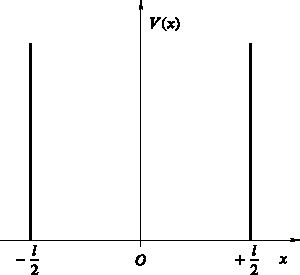
\includegraphics{figure/fig06.13}
  \caption{无限深的方势阱}
  \label{fig:06.13}
\end{wrapfigure}
当质点在位于$ x = \pm \dfrac { l } { 2 } $
的两个刚性壁之间运动时,它的势能函数就近似是一方
势阱。在这种势能函数下,无论什么能量,运动都是
束缚的,运动范围限制在
$ - \dfrac { l } { 2 } \leqslant x \leqslant \dfrac { l } { 2 }   $之间它的运
动周期,按式\eqref{eqn:06.05.07}可以
求得为

\begin{equation*}
  T = \sqrt { \frac { 2 m } { E } } \int _ { - \frac { l } { 2 } } ^ { \frac { l } { 2 } } \dif x = \sqrt { \frac { 2 m } { E } } l
\end{equation*}
在运动范围中,$ V = 0   $,所以$ E = \dfrac { 1 } { 2 } m v ^ { 2 }   $,因此上式还可以写成
\begin{equation*}
  T = \frac { 2 l } { v }
\end{equation*}
这个结果是显然的,它表示以速度$ v $运动的质点来回一周所需的
% 187.jpg
时间。

\clearpage
\example 注意第五章的式\eqref{eqn:05.05.07},即
\begin{equation}\label{eqn:06.05.08}
  \left[ \frac { 1 } { R _ { 0 } } \left( \frac { \dif R } { \dif t } \right) \right] ^ { 2 }- \frac { 8 \uppi G } { 3 } \rho _ 0 \frac { 1 } { \left( \dfrac { R } { R _ { 0 } } \right) } = K
\end{equation}
它在形式上与式\eqref{eqn:06.05.02}是相似的,现在$ R $相当于$ x $,式中第一项
相当于宇宙膨胀的动能,第二项是引力势能,而$ K $是“总能”。
我们在第五章中已指出,当$  K < 0   $时,宇宙膨胀将来会停止,而变
成收缩。

从一维运动的观点看,由式\eqref{eqn:06.05.08}所描写的一维运动,当$ K
  <0 $时是束缚的运动。因此,我们可以计算$ R $从0增大到$ R_{\max} $(相当
于整个宇宙膨胀阶段)再从$ R_{\max} $回到0(相当于将来发生的宇宙收
缩阶段)整个需要多少时间。利用类似于推求式\eqref{eqn:06.05.07}的方法,
可以推求出宇宙完成一个膨胀收缩循环的时间为
\begin{equation}\label{eqn:06.05.09}
  t = 2 \frac { 1 } { R _ { 0 } } \int _ 0 ^ { R _ { \max } } \frac { \dif R } { \sqrt { \dfrac { 8 \uppi G } { 3 } \rho _ { 0 } R _ { 0 } \dfrac { 1 } { R } - | K | } }
\end{equation}
其中
\begin{equation*}
  R _ { \max } = \frac { 8 \uppi G \rho _ { 0 } R _ { 0 } } { 3 | K | }
\end{equation*}
作变量代换
\begin{equation*}
  R ' = \frac { R } { \left( \dfrac { 4 \uppi G \rho _ { 0 } R _ { 0 } } { 3 | K | } \right) }
\end{equation*}
式\eqref{eqn:06.05.09}成为
\begin{equation}\label{eqn:06.05.10}
  \begin{aligned}
    t & = \frac { 8 \uppi G \rho _ { 0 } } { 3 { | K | } ^ { 3 / 2 } } \int _ { 0 } ^ { 2 } \frac { \dif R '  } { \sqrt { \dfrac { 2 } { R ' } - 1 } } \\
      & = \uppi \frac { 8 \uppi G \rho _ { 0 } } { 3 { | K | } ^ { 3 / 2 } }
  \end{aligned}
\end{equation}
% 188.jpg
如果我们当今宇宙中的平均质量密度$ \rho _ 0 $是临界密度$ \rho _ c $的2倍,即
\begin{equation}\label{eqn:06.05.11}
  \rho _ { 0 } = 2 \rho _ { c } = 2 \frac { 3 H _ 0 ^ { 2 } } { 8 \uppi G }
\end{equation}
则由式\eqref{eqn:05.05.12}有
\begin{equation}\label{eqn:06.05.12}
  K = - H _ { 0 } ^ { 2 }
\end{equation}
将式\eqref{eqn:06.05.11}及式\eqref{eqn:06.05.12}代入式 \eqref{eqn:06.05.10},得到
\begin{equation}\label{eqn:06.05.13}
  t = 2 \uppi \frac { 1 } { H _ { 0 } }
\end{equation}
再利用式\eqref{eqn:05.04.06}给出的观测值$ H _ { 0 } $就得到
\begin{equation*}
  t \approx 1.26 \times 10 ^ { 11 } \text{年}
\end{equation*}
这就是宇宙的演化时间尺度。